%%%%%%%%%%%%%%%%%%%%%%%%%%%%%%%%%%%%%%%%%%%%%%%%%%%%%%%%%%%%%%%%%%%%%%
% How to use writeLaTeX: 
%
% You edit the source code here on the left, and the preview on the
% right shows you the result within a few seconds.
%
% Bookmark this page and share the URL with your co-authors. They can
% edit at the same time!
%
% You can upload figures, bibliographies, custom classes and
% styles using the files menu.
%
% If you're new to LaTeX, the wikibook is a great place to start:
% http://en.wikibooks.org/wiki/LaTeX
%
%%%%%%%%%%%%%%%%%%%%%%%%%%%%%%%%%%%%%%%%%%%%%%%%%%%%%%%%%%%%%%%%%%%%%%
\documentclass{tufte-handout}
%\usepackage{thmtools}

%\geometry{showframe}% for debugging purposes -- displays the margins

\usepackage{amsmath}

% Set up the images/graphics package
\usepackage{graphicx}
\setkeys{Gin}{width=\linewidth,totalheight=\textheight,keepaspectratio}
\graphicspath{{graphics/}}

\title[Lecture 4]{\large AI2100/EE5609 Convex Optimization Theory \\ \LARGE Lecture 4: Polyhedra,  Norm Balls, Norm Cones}
\author[Aditya S]{Scribe(s): Athira Krishnan R, Tadipatri Uday Kiran Reddy}
\date{\today}  % if the \date{} command is left out,\section{Norm Ball}

%  the current date will be used

% The following package makes prettier tables.  We're all about the bling!
\usepackage{booktabs}
\usepackage{amsmath, amsthm, amssymb, bm}
\usepackage{tikz, pgfplots}
\usetikzlibrary{shapes, arrows, positioning, fit, calc}   
\tikzset{block/.style={draw, thick, text width=1.2cm ,minimum height=0.8cm, align=center},   
line/.style={-latex}     
} 

\newtheorem{theorem}{Theorem}
\theoremstyle{remark}
\newtheorem*{defn}{Definition}
\renewcommand{\vec}[1]{\underline{#1}}
% The units package provides nice, non-stacked fractions and better spacing
% for units.
\usepackage{units}

% The fancyvrb package lets us customize the formatting of verbatim
% environments.  We use a slightly smaller font.
\usepackage{fancyvrb}
\fvset{fontsize=\normalsize}

% Small sections of multiple columns
\usepackage{multicol}

% Provides paragraphs of dummy text
\usepackage{lipsum}

% These commands are used to pretty-print LaTeX commands
\newcommand{\doccmd}[1]{\texttt{\textbackslash#1}}% command name -- adds backslash automatically
\newcommand{\docopt}[1]{\ensuremath{\langle}\textrm{\textit{#1}}\ensuremath{\rangle}}% optional command argument
\newcommand{\docarg}[1]{\textrm{\textit{#1}}}% (required) command argument
\newenvironment{docspec}{\begin{quote}\noindent}{\end{quote}}% command specification environment
\newcommand{\docenv}[1]{\textsf{#1}}% environment name
\newcommand{\docpkg}[1]{\texttt{#1}}% package name
\newcommand{\doccls}[1]{\texttt{#1}}% document class name
\newcommand{\docclsopt}[1]{\texttt{#1}}% document class option name

\begin{document}

\maketitle% this prints the handout title, author, and date
\fancyhead[L]{AI2100/EE5609}
%\begin{abstract}
%\noindent This document describes the Tufte handout \LaTeX\ document style.
%It also provides examples and comments on the style's use.  Only a brief
%overview is presented here; for a complete reference, see the sample book.
%\end{abstract}
\newthought{Crisp Summary}
%\printclassoptions
\begin{itemize}
    \item Convex sets are set which have clear line of sight between any two points on the set. Line segment joining any two points in the set completely lies in the set.
    \item A set $\mathbb{C}$ $\epsilon$ $\mathbb{R}^n$ is affine if the line through 2 distinct points in \mathbb{C} lies in $\mathbb{C}$.
    \item For convex problems local minima and global minima coincides.
    \item Intersection of convex sets are convex.
    \item If a set is convex, so are its affine combination, perspective and inverse perspective transformations.
\end{itemize}
% \newthought{Recall:} vector spaces, matrix multiplication, linear independence
\section{Hyperplane}
\marginnote{ For example, \{\vec{x}:x1+3x2+x3=5\} is a plane in $\mathbb{R}^3$. This can be written in the form $\{x:a\mathcal{\vec{X}}=b\}$. This being a linear combination of x is therefore affine combination and convex.}
\cite{boyd2004convex}A hyperplane is the set of the form, $\{x|a^\top x=b\}$, where a $\epsilon$ $\mathbb{R}^n$, $a\neq0$ and  b $\epsilon$ $\mathbb{R}$. Geometrically it can be interpreted as the set of points with a constant inner product to a given vector \vec{a} or as a hyperplane with normal vector a and constant b determines the offset of the hyperplane from the origin. This can be expressed in the form, $\{x| a^\top(x-x0)=0\}$ where x0 is any point in the hyperplane. 
\section{Halfspaces}
A hyperplane divides $\mathbb{R}^n$ space into 2 half spaces. A half space is a set of the form $\{x|a^\top x \ge b\}$, where $a \neq 0$. Halfspaces are convex but not affine.

\begin{marginfigure}
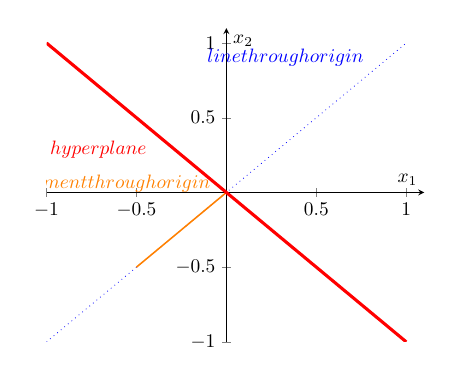
\begin{tikzpicture}[scale=0.7]
    \begin{axis}[
        axis lines=center,
        xmax = 1.1,
        ymax = 1.1,
        ylabel=$x_2$,
        xlabel=$x_1$,
        ]
        \addplot [domain=-1:1,samples=250,  dotted , blue] {x}
            node [pos=0.9, above left] {$line through origin$};
        \addplot [domain=-0.5:0,samples=250,  thick , orange] {x}
            node [pos=0.9, above left] {$line segment through origin$};
        \addplot [domain=-1:1,samples=250, ultra thick, red ] {-x}
            node [pos=0.3, below left] {$hyperplane$};
        % \filldraw[black] (0,0)
        
    \end{axis}
        \end{tikzpicture}
\caption{Hyperplane shown in red line separates the $\mathbb{R}^2$ plane into two. For a point in hyperplane set, say origin, line segment between 2 points lies inside the halfplane but the line through them may not. So by definition, hyperplane is convex but not affine.}

\end{marginfigure}
Half spaces can also be represented as $\{x|a^\top (x-x0) \le 0\}$, where x0 is any point on the associated hyperplane.
\section{Polyhedron}
A polyhedron is defined as the solution set of a finite number of linear equalities and inequalities. Or a polyhedra is an intersection of halfspaces and hyperplanes. Affine sets, rays, line segments half spaces are few examples of polyhedra. Since halfspaces and hyperplanes are convex, so is polyhedra. A polyhedra need not be bounded. A bounded polyhedra is also reffered as "polytope". A polyhedra can be represented in the form, $\mathbb{P}=\{x| \mathcal{A}x \le b, \mathcal{C}x=d\}$.
\begin{marginfigure}
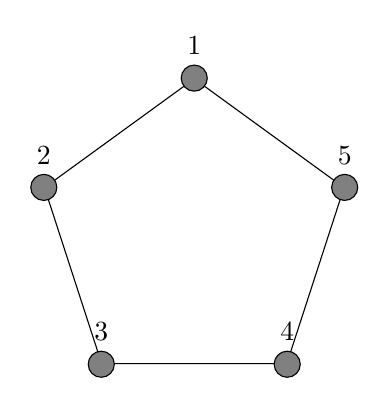
\begin{tikzpicture}[scale=0.7]
\node[minimum size=4cm,draw,regular polygon,regular polygon sides=5,fill=white] (a) {};
\foreach \i in {1,...,5}
    \node[circle,radius=.1cm,draw,
    label=above:{$\i$},
    fill=gray] at (a.corner \i) {};
\end{tikzpicture}
\caption{Polytope formed by intersection of 5 halfspaces or 5 vertices.}
\end{marginfigure}
Polytope can be seen also as a convex hull formed by its vertices.
Therefore a polytope can be represented in terms of edges as $\{x|\mathcal{A}\vec{x}  \le b\}$ or of vertices as $\{x|\sum_{i=1}^N\theta_i\mathbf{v}_i\}$.
In computing the polytope using edge representation, in nD space number of planes required will be 2n, whereas in case of vertex based method, $2^n$ vertices would be required. Therefore as number of vertices increases, more would be the computation.
\subsection{Simplex}
It is a polyhedra formed by a certain number of non degenerates.\cite{boyd2004convex} Consider k+1 points $\vec{v}_1, \vec{v}_2, \ldots, \vec{v}_k \epsilon \mathbb{R}^n $ are affinely independent. Or in simple terms,
$\vec{v}_1-\vec{v}_0, \ldots, \vec{v}_k-\vec{v}_0$ are linearly independent. Now taking convex hull of all these points results in a simplex represented in the form, $\mathcal{C}=conv\{\vec{v}_0, \ldots, \vec{v}_k\}=\{\theta_0\vec{v}_0+\ldots+\theta_k\vec{v}_k\theta \ge 0, 1^\top\theta=1\}$

\marginnote{Minimum number of points in 3D to construct a polyhedra is 4, whereas its 3 in 2D. }\\
\usepgfplotslibrary{fillbetween}
\begin{figure}
    \centering


\begin{tikzpicture}[scale=0.7]
    \begin{axis}[
        axis lines=center,
        xmax = 1.1,
        ymax = 1.1,
        ylabel=$x_2$,
        xlabel=$x_1$,
        ]
        \addplot [name path = A,domain=0:1,samples=250,  dotted , blue] {0.5*x}
            node [pos=0.9, above right] {$\vec{v}_1$};
        \addplot [name path = B,domain=0:0.2,samples=250,  thick , orange] {4*x}
            node [pos=0.1, above right] {$\vec{v}_2$};
        \addplot[red!10, opacity=0.4] fill between[of=A and B];
        % \addplot [domain=0.2:1,samples=250, ultra thick, red ] {4.5*x-0.5}
        %     node [pos=0.3, above right] {$hyperplane$};
        % \filldraw[black] (0,0)
        
    \end{axis}

\end{tikzpicture}
\caption{Polytope using 2 linearly independent vectors.}
\end{figure}
Consider the set, $\{xx \ge 0, 1^\top x=1 \}$ (simplex polyhedra). Ensure they sum to 1 and is non negative.
Let the probability vector be $\{x:\vec{x1,x2} \ge 0 x1+x2=1 \}$. $\vec{v}_0=0$,....$\vec{v}_i=ei$. Simplex would be as shown below.
\begin{figure}
    \centering
\begin{tikzpicture}[scale=0.7]
    \begin{axis}[
        axis lines=center,
        xmax = 1.1,
        ymax = 1.1,
        ylabel=$x_2$,
        xlabel=$x_1$,
        ]
        \addplot [name path = A,domain=0:1,samples=250,  dotted , blue] {-1*x+1}
            node [pos=0.9, above right] {};
        \addplot [name path = B,domain=0:1,samples=250,  thick ,black] {0}
            node [pos=0.1, above right] {};
        \addplot[red!10, opacity=0.4] fill between[of=A and B];
        % \addplot [domain=0.2:1,samples=250, ultra thick, red ] {4.5*x-0.5}
        %     node [pos=0.3, above right] {$hyperplane$};
        % \filldraw[black] (0,0)
        
    \end{axis}

\end{tikzpicture}\\
\caption{Polytope using 2 linearly independent vectors.}
\end{figure}
Consider  bounded polyhedron or a polytope P. Consider the optimization problem,\\
$min(a^\top x) $\\
subject to $ \vec{x} \epsilon P$
This is a convex problem as its constraints set is convex and objective function $a^\top x$ being a linear combination. Being convex, the local minima and global minima of the problem coincides. So optima falls to one of the vertices of the polyhedra. If  $a^\top v1=-1$, $a^\top v2=-1$ the any point on the line segment joining v1 and v2, $a^\top (\theta v1+(1-\theta)v2=-1$.
\begin{proof}
Taking the convex combination of all n vertices $v_1,v_2.....v_n$, is given by,\\
$a^\top(\sum_{i=1}^N \theta_i v_i)$, $0 \le \theta \le 1  $ and $\sum_{i=1}^N \theta_i=1$
As weighted average >smallest element in the set,\\
$a^\top(\sum_{i=1}^N \theta_i v_i) \ge min_{i1}^N\theta_i v_i$
Then value in the function would be atleast $a^\top v_i$ or value at the vertices. Therefore one of the vertices is an optima.
\end{proof}
\begin{marginfigure}
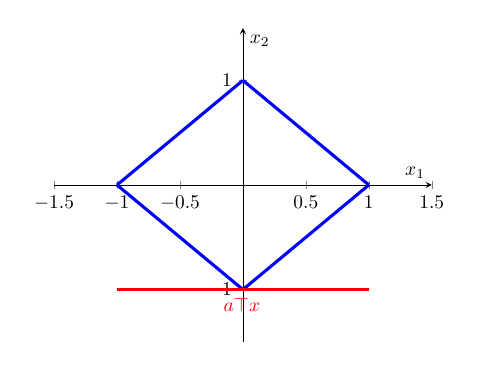
\begin{tikzpicture}[scale=0.7]
\begin{axis}[
        axis lines=center,
        xmax = 1.5,
        xmin=-1.5,
        ymin=-1.5,
        ymax = 1.5,
        ylabel=$x_2$,
        xlabel=$x_1$,
        ]
        \addplot [domain=-1:0,samples=250,  ultra thick , blue] {x+1}
            node [pos=0.9, above left] {};
        \addplot [domain=0:1,samples=250,  ultra thick , blue] {1-x}
            node [pos=0.9, above left] {};
        \addplot [domain=1:0,samples=250, ultra thick, blue ] {-1+x}
            node [pos=0.3, below left] {};
        \addplot [domain=0:-1,samples=250, ultra thick, blue ] {-1-x}
            node [pos=0.3, below left] {};
        % \filldraw[black] (0,0)
        \addplot[ultra thick, samples=250, smooth,domain=-1:1,red] coordinates {(-1,-1)(1,-1)}node [pos=0.6, below left] {$a\top x$};

        
\end{axis}
\end{tikzpicture}
\caption{Minima of polyhedra occurs at one of its vertex}
\end{marginfigure}
\section{Norm Ball}
 In mathematics, a norm is the length (or size) of a vector from origin.
A function to be called as norm, it need to have following properties,
\begin{enumerate}
    \item $||X| \ge 0$, norm of any vector is non negative. $||X||=0$, iff $X=0$.
    \item $||\alpha X||=\alpha||X||$, norm follows property of homogeniety.
    \item ||X+Y|| \le ||X||+||Y||, nonrm follows triangle inequality.
\end{enumerate}

A Lp-norm is a norm on a finite-dimensional space of dimension N defined as, $||u||_p=(\sum_{i=1}^N|u_i|^p)^{1/p}$, where p \ge 1. This set can be represented as $\{x| ||X|| \le r\}$, where r is a constant. For p<1, convexity is not valid.
The norm for p=1 is the sum of the distances a 3D computer numerical control (CNC) mill would have to move in the x,y,z directions. In 3D L1 unit norm ball takes shape of an octahedron, whereas in 2D it forms a square shape.It can be defined as 1 norm: $\{x| |x1|+x2| \le r\}$. When p=2, norm deduces to eucledian distance (Line of sight distance), now unit norm ball takes a circle shape. It can be represented as 2 norm : $\{x| x1^2+x2^2 \le r^2\}$.
When p=$\infty$, norm is computed as $||u_\inf=max\{u_i\}$.
\begin{theorem}
Norm balls are convex.
\end{theorem}
\begin{proof}

Consider 2 points in set X, such that ||X1|| \le r and ||X2|| \le r. Then by triangular inequality, 
$||\theta x1+(1-\theta)x2|| \le ||\theta x1||+||\theta x2||$
Since $\theta $ is a scalar,by scalar multiplication,
$||\theta x1+(1-\theta)x2|| \le \theta|| x1||+\theta|| x2||$
By definition,
$||\theta x1+(1-\theta)x2|| \le \theta r+\theta r  \le r$
Therefore norm balls are also convex.
\end{proof}
\begin{theorem}
Given transformation matrix P is positive semi definite, Norm balls preserves convexity during stretching/compressing the set.
\end{theorem}
\begin{proof}
Consider a convex set $\{x| x^top.x \le 1\}$ representing 2 norm. ${x|vec{x}^\top P^{-1} \vec{x}}$, assuming $P^{-1}$ is symmetric. By spectral decomposition theorem, $P=VDV^\top$. By taking inverse on both sides, $P^-1=VD^{-1}V^\top$, then set x can be rewritten as,
$\{x| x^\top VD^{-1}V^\top x \le 1\}$.
Taking $V^\top x$ as y,problem reduces to form, $\{y|y^\top D^-1y \le 1\}$. $D=\begin{bmatrix} 
	\lambda1 & 0&... & 0 \\
	0 & \lambda2 & ...&0\\
	. & . & ...&.\\
	. & . & ...&.\\
	0&0&...&\lambda n\\
	\end{bmatrix}$
	Assuming all $\lambda_i>0$, solution deduces to form,
	$\{y|\sum_{i=1}^N y_i^2/\lambda_i^2 \}$. This represents an ellipsoid in 2D of the form, $y1^2/a^2+y2^2/b^2 \le 1$. Therefore given that P is positive semi definite, even after stretching or compressing the set remains convex.


\end{proof}
\marginnote{Sketch 1 norm and infinite norm balls}
\begin{marginfigure}
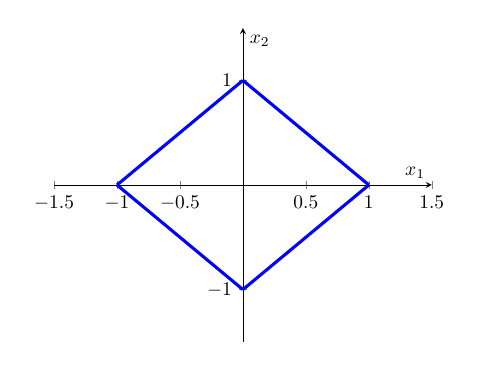
\begin{tikzpicture}[scale=0.7]
\begin{axis}[
        axis lines=center,
        xmax = 1.5,
        xmin=-1.5,
        ymin=-1.5,
        ymax = 1.5,
        ylabel=$x_2$,
        xlabel=$x_1$,
        ]
        \addplot [domain=-1:0,samples=250,  ultra thick , blue] {x+1}
            node [pos=0.9, above left] {};
        \addplot [domain=0:1,samples=250,  ultra thick , blue] {1-x}
            node [pos=0.9, above left] {};
        \addplot [domain=1:0,samples=250, ultra thick, blue ] {-1+x}
            node [pos=0.3, below left] {};
        \addplot [domain=0:-1,samples=250, ultra thick, blue ] {-1-x}
            node [pos=0.3, below left] {};
        % \filldraw[black] (0,0)
        
\end{axis}
\end{tikzpicture}
\caption{1 norm ball.}
\end{marginfigure}

\begin{marginfigure}
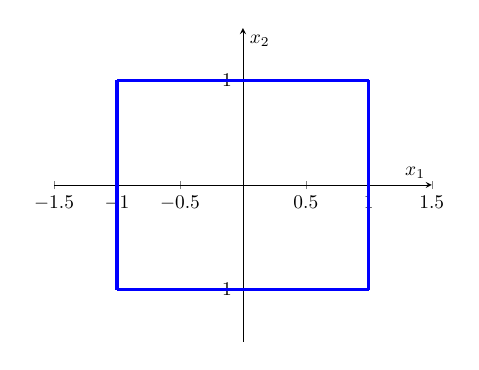
\begin{tikzpicture}[scale=0.7]
\begin{axis}[
        axis lines=center,
        xmax = 1.5,
        xmin=-1.5,
        ymin=-1.5,
        ymax = 1.5,
        ylabel=$x_2$,
        xlabel=$x_1$,
        ]
        \addplot [domain=-1:1,samples=250,  ultra thick , blue] {1};
            % node [pos=0.9, above left] {};
        \addplot[ultra thick, samples=250, smooth,domain=0:1,blue] coordinates {(1,1)(1,-1)};
        \addplot [domain=-1:1,samples=250, ultra thick, blue ] {-1};
        \addplot[ultra thick, samples=250, smooth,domain=-1:0,blue] coordinates {(-1,1)(-1,-1)};


\end{axis}
% \draw (0,0) -- (1,0) -- (1,1) -- (0,1) -- cycle;
\end{tikzpicture}
\caption{infinite norm ball.}
\end{marginfigure}
\section{Norm Cones}
Set $\mathbb{C}$ is a cone if for any  $x \epsilon \mathbb{C}$, $\theta x \epsilon \mathbb{C}$ for any $\theta \ge 0$. $\theta x$ represents the line joining x and origin or in other words, it represents ray pointing in the direction of x from origin. For any point in C the ray lies in C. Cones are convex sets.
In $\mathbb{R}^2$, cones are represented as $z=\sqrt{x^2+y^2}$= L2 norm of first 2 coordinates. As any point on the cone is given by $z=\sqrt{x^2+y^2}$, any point inside the cone can be represented as $z \ge \sqrt{x^2+y^2}$. Therefore in $\mathbb{R}^n$, norm of top n-1 coordinate $ \le  n^{th}$ coordinate. In $\mathbb{R}^{n+1}$ a cone is $\{ (x,t)| x\epsilon \mathbb{R}^{n},t\epsilon \mathbb{R},||x|| \le t\}$. 2 norm cones are generally referred as Lorentz cones. All norm cones are convex.
\begin{proof}
Assume a set $\{ (x,t)| x\epsilon \mathbb{R}^{n},t\epsilon \mathbb{R},||x|| \le t\}$, then ||x|| \le t, this means, $||x|/t \le 1$. This represents the perspective transform of (x,t). This is of the form $||X|| \le 1$. As norm is convex, so is norm cones.\\
\textit{Question}.\\
Consider a set in $\mathbb{R}^n $ given by $\{ x:x^\top P^{-1}x \le (\mathbb{C}^\top x)^2,\mathbb{C}^\top x>0\}$. Assume P is positive definite, $S_{++}^n$. Let a new variable $t= \mathbb{C}.^\top x$, set becomes $\{x:x^\top P^{-1}x \le t^2,t>0,t=\mathbb{C}.^\top x \}$\\
Taking square root on both sides,
$\{x: \sqrt{x^\top P^{-1}x}  \le t,t>0,t=\mathbb{C}.^\top x\}$\\
When last coordinate is positive and $t=\mathbb{C}.^\top x$, this becomes equivalent to linear combination of first n values, this represents a hyperplane. \\If $\sqrt{x^\top P^{-1}x}  \le t$ is convex (being a hyperplane), rest also becomes convex. Assume $P=VDV^\top$ is symmetric positive definite matrix, then $x^topVD^{1/2} D^{1/2}V^top x$.\\ If $y= D^{1/2}V^top x$, this reduces to $\sqrt{y^\top y \le t}$, which means $||y|| \le t$, represents a cone.\\ Therefore a norm cone is convex it is intersection of hyperplane and cone.
\end{proof}
% \textit{Question}.\\
% Consider the set in $\mathbb{R}^n$ given by $\{\overline{x}: \overline{x}^TP^{-1}\overline{x} \le (\overline{c}^T\overline{x})^2, \overline{c}^T\overline{x} > 0\}$ where $P$ is positive defnite $P \in {\$}^n_{++}$.\\ \\\
% The above set can also be written as $\{\overline{x}: \overline{x}^TP^{-1}\overline{x} \le t^2, t > 0, t = \overline{c}^T\overline{x}\}$. Now by applying Singular Value Decomposition(SVD), we get $P=VDV^T$.
% \begin{gather*}
%     \{\overline{x}: \overline{x}^T(VDV^T)^{-1}\overline{x} \le t^2, t > 0, t = \overline{c}^T\overline{x}\}\\
%     \{\overline{x}: \overline{x}^TVD^{-1}V^T\overline{x} \le t^2, t > 0, t = \overline{c}^T\overline{x}\} (\text{ $\because$ Since $V$ is orthonormal matrix})\\
%     \left \{\begin{pmatrix} \overline{x} \\ t \end{pmatrix} : \left(\frac{V^T\overline{x}}{t}\right)^TD^{-1}\left(\frac{V^T\overline{x}}{t}\right) \le 1, t > 0, t = \overline{c}^T\overline{x}\right \}
% \end{gather*}



%\bibliography{references}
%\bibliographystyle{plainnat}

\section{Separating hyperplane theorem}
Suppose $C_1$ and $C_2$ are nonempty disjoint convex sets, i.e, $C_1 \cap C_2 \in \Phi$. Then there exists $\overline{a} \neq 0$ and $b$ such that $\overline{a}^T\overline{x} \le b; \forall \overline{x} \in C_1$ and $\overline{a}^T\overline{x} \ge b; \forall \overline{x} \in C_2$. The hyperplane $\{\overline{x} | \overline{a}^T\overline{x} = b\}$ is called \textit{separating hyperplane} for the sets $C_1$ and $C_2$.\\
\begin{proof}
    Take $\overline{a} \in C_1$ and $\overline{b} \in C_2$ such that these two vectors form a pair that belongs to the set $inf\{||\overline{u}-\overline{v}||_2 ; \overline{u} \in C_1, \overline{v} \in C_2\}$ \\
    Then we have to show that affine function $f(\overline{x}) = \overline{c}^T\overline{x} - d$ is the separating hyperplane such that $\overline{c} = \overline{a} - \overline{b}$ and $d = \frac{||a||_2^2 - ||b||_2^2}{2}$.\\
    Now since f is non-negative on $C_1$ and non-positive on $C_2$, Suppose there is point $\overline{u} \in C_1$ such that $f(\overline{u}) < 0$.\\
    \begin{gather*}
        f(\overline{u}) = (\overline{a} - \overline{b})^T\overline{u} - \frac{||a||_2^2 - ||b||_2^2}{2} = (\overline{a} - \overline{b})^T(\overline{u}-\overline{b}) + 0.5||\overline{d}-\overline{c}||_2^2\\
        (\overline{a} - \overline{b})^T(\overline{u}-\overline{a}) < 0\\
        (\overline{b} - \overline{a})^T(\overline{u}-\overline{a}) > 0
    \end{gather*}
    The above inequality means that some point in $C_1$ makes acute angle with line joining closed of two sets which possible only when $\overline{u}$ is more closer to $\overline{b}$ than $\overline{a}$ is. As $\overline{a}$ itself is closest thus, such a $\overline{u}$ cannot exists.
\end{proof}
\begin{marginfigure}
\begin{tikzpicture}[scale=0.7]
\begin{axis}[
        axis lines = left,
        xmin=-3, xmax=3, ymin=-3, ymax=3,
        axis equal,
        xlabel = $x_1$,
        ylabel = {$x_2$},
        yticklabels={,,}
        ]
        \draw (axis cs: -1.5, 0) circle [radius=100, red];% I've set the radius to 10 only for better show the image
        \draw (axis cs: 1.5, 0) circle [radius=100, blue];% I've set the radius to 10 only for better show the image
        \addplot[ultra thick, samples=250, smooth,domain=-1:0,green] coordinates {(0, 2)(0, -2)};
    \end{axis}
% \draw (0,0) -- (1,0) -- (1,1) -- (0,1) -- cycle;
\end{tikzpicture}
\caption{Seperating hyperplane}
\end{marginfigure}
\textit{Property}: Every (closed) convex set has a unique point with smallest norm.\\

\section{Supporting hyperplane theorem}
Take a point on the boundary of a convex set, drawing tangent through it will make the whole convex set lie on only one side of the line.
\begin{marginfigure}
\begin{tikzpicture}[scale=0.7]
\begin{axis}[
        axis lines = left,
        xmin=-3, xmax=3, ymin=-3, ymax=3,
        axis equal,
        xlabel = $x_1$,
        ylabel = {$x_2$},
        yticklabels={,,}
        ]
        \draw (axis cs: -1.5, 0) circle [radius=100, red];
        \addplot[ultra thick, samples=250, smooth,domain=-1:0,green] coordinates {(-3, -1)(3, -1)};
    \end{axis}
% \draw (0,0) -- (1,0) -- (1,1) -- (0,1) -- cycle;
\end{tikzpicture}
\caption{Supporting hyperplane}
\end{marginfigure}
\section{Farkas Lemma}
Consider the below two statements,\\
\begin{enumerate}
    \item We can find $\overline{x} \ge \overline{0}$ such that $\mathbf{A}\overline{x} = \overline{b}$.
    \item We cam find $\overline{a}$ such that $\overline{a}^T\overline{b} \ge 0$ ans $\mathbf{A}^T\overline{a} \le \overline{0}$
\end{enumerate}
Farkas lemma states that exactly only one of the above statements is true.
\begin{proof}
    Let $\overline{x} \ge \overline{0}$, s.t $\mathbf{A}\overline{x} = \overline{b}$ then,
    \begin{gather*}
        \overline{a}^T\mathbf{A}\overline{x} = \overline{a}^T\overline{b}\\
        \implies (\mathbf{A}^T\overline{a})^T\overline{x} = \overline{a}^T\overline{b}
    \end{gather*}
    \textit{Assume Statement 1) is true}.\\
    Let $\overline{a}^T\overline{b} > 0$, then not all entries of $(\mathbf{A}^T\overline{a})^T$ are negative which means that statement 2) is false.\\ \ \\
    \textit{Assume Statement 2) is true}.\\
    Then we cannot have all entries of $\overline{x}$ to be positive some of them must be negative to satisfy the above equation.\\
    Thus Both Statement 1) and 2) cannot be true together.\\ \\\
    We can also show this result using separating hyperplane theorem take convex set $C_1 = \{\mathbf{A}\overline{x}: \overline{x} \ge 0\}$, this set is cone. And another set $C_2 = \{\overline{b}\}$. Now we can always find a hyper plane which separates these two sets, note that set $C_1$ is infinite set thus plane can never form a acute angle. Thus plane would be oriented towards $\overline{b}$. 
\end{proof}
\begin{marginfigure}
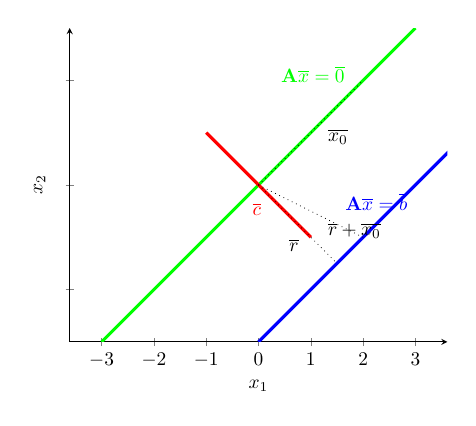
\begin{tikzpicture}[scale=0.7]
\begin{axis}[
        axis lines = left,
        xmin=-3, xmax=3, ymin=-3, ymax=3,
        axis equal,
        xlabel = $x_1$,
        ylabel = {$x_2$},
        yticklabels={,,}
        ]
        \addplot[ultra thick, samples=250, smooth,domain=-1:0,green] coordinates {(-3, -3)(3, 3)}node [pos=0.8
        , above left] {$\mathbf{A}\overline{x} = \overline{0}$};
         \addplot[ultra thick, samples=250, smooth,domain=-1:0,blue] coordinates {(0, -3)(5, 2)}node [pos=0.6
        , below left] {$\mathbf{A}\overline{x} = \overline{b}$};
        \addplot[ultra thick, samples=250, smooth,domain=-1:0,red] coordinates {(-1, 1)(1, -1)}node [pos=0.6, below left] {$\overline{c}$};
        \addplot[dotted, samples=250, smooth,domain=-1:0,black] coordinates {(0, 0)(1.5, -1.5)}node [pos=0.6, below left] {$\overline{r}$};
        \addplot[dotted, samples=250, smooth,domain=-1:0,black] coordinates {(0, 0)(2, 2)}node [pos=0.6, below right] {$\overline{x_0}$};
        \addplot[dotted, samples=250, smooth,domain=-1:0,black] coordinates {(0, 0)(2, -1)}node [pos=0.6, below right] {$\overline{r} + \overline{x_0}$};
        
    \end{axis}
% \draw (0,0) -- (1,0) -- (1,1) -- (0,1) -- cycle;
\end{tikzpicture}
\caption{Linear optimisation problem}
\end{marginfigure}
\textit{Problem}\\
Consider the following optimisation problem,\\
min $\overline{c}^T\overline{x}$ \\
such that $\mathbf{A}\overline{x} = \overline{b}$\\ \ \\
\textit{Solution}\\
Let $\overline{r}$ satisfy $\mathbf{A}\overline{r} = \overline{b}$, then general solution of the above equation is $\overline{r} + \overline{x_0}$ where $\overline{x_0}$ is in null space of $\mathbf{A}$. This means that solutions to the equation is just null space shifted by $\overline{r}$. If $\overline{c}$ is perpendicular to null space of then $\overline{c}^T\overline{x} = \overline{c}^T\overline{r} + \overline{x_0} = \overline{c}^T\overline{r}$. If $\overline{c}$ is not perpendicular to null space then value is $-\infty$.

\section{Linear programming problem}
min $\overline{c}^T\overline{x}$\\
such that $\mathbf{A}\overline{x} = \overline{b}$ and $\overline{x} \ge 0$\\ \ \\
Any linear programming problem can be boiled down to above optimisation problem. As a consequence of farkas lemma we can show that there can exists a solution to above problem otherwise we can give a certificate that above problem has no such $\overline{x}$ which satisfies the above problem.

\subsection{Ordering of Vectors}
If $\overline{x} < \overline{y}$ then $\overline{y}-\overline{x} \in \mathcal{K}$, where $\mathcal{K}$ is a cone. Ordering changes with the choice of the cone. We usually consider first quadrant of $\mathbb{R}^2$ as our choice of cone.\\
We can always find a pair of vectors where both $\overline{x}-\overline{y}$ and $\overline{y}-\overline{x} \not\in \mathcal{K}$, such vectors are not comparable and every choice of cone can such pairs.
\end{document}